%!TEX root = ../dissertation.tex

\section{Camera Model}
\label{cha2:cameramodel}

In this section, are introduced the essential concepts on the pinhole camera model that follow. Digital cameras are equipped with a sensor (mostly charge-coupled devices, CCD, and CMOS') that transforms light into discrete electrical signals. When taking a picture, some of the light reflecting on the object is directed towards the camera pinhole (tiny aperture on the camera), forming a 180º inverted image of the object on the sensor, as shows on Figure \ref{cha2:sec2:fig:camera_concepts}. All the light rays entering the camera converge into the pinhole and diverge on the other side (with a unique one-to-one correspondence). Therefore the pinhole is also named the \textbf{center of projection}, principal point, or focal point.

In cameras the aperture size and light-exposure time can be controlled. A smaller aperture produces a sharper image but needs a longer exposure time to collect enough light, whereas a larger aperture allows more light to be captured, but at the expense of producing blurred images.

The image of the object is projected onto the so-called \textbf{image plane}. When moving this plane closer to the pinhole (zoom out), the projected object gets smaller, and vice-versa. The distance between the plane and the aperture is the \textbf{focal length}, or focal distance. The view-angle of a camera depends on the focal distance, and on the sensor size. The image resolution depends solely on the number of pixels that fit on the sensor.

A useful coordinate system, called the \textbf{camera reference system}, is centered at the pinhole, and has its z-axis perpendicular to the image plane, as mentioned in section \ref{cha2:represent}. The line defined between the center of projection and the center of the image plane is called the \textbf{optical axis}.

\begin{figure}[ht]
	\centering
	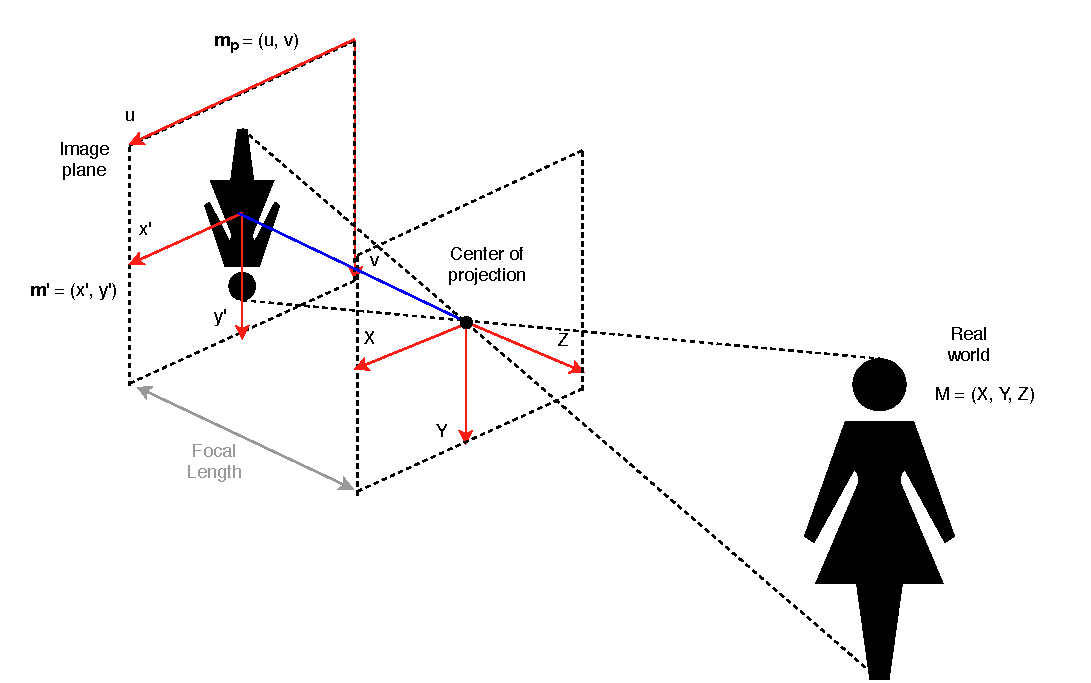
\includegraphics[width=\textwidth]{images/cameraconcepts.pdf}
	\caption[Pinhole Camera Model]{Pinhole Camera Model. The girl defined by the generic set of points $M$ is projected onto the image plane (defined by the set of generic points $\bf m_{p}$) through the light rays passing by the camera's pinhole, called the center of projection. The focal length is the distance from the center of the image plane to the center of projection. The digital image's coordinate system $(u, v)$ is defined on top right (CHECK THIS) corner of the image. The optical axis is the blue line.}
	\label{cha2:sec2:fig:camera_concepts}
\end{figure}

Figure \ref{cha2:sec2:fig:camera_concepts} summarizes the concepts explained above, and helps at understanding the upcoming details. It's possible to establish a relationship between a real point in space and a point in an image in pixels, through the camera model as follows.

\begin{enumerate}
	\item \textbf{Passing from the world frame to the camera reference frame}
	
	An arbitrary real point in space $M_W = [X_W \ Y_W \ Z_W]^T$ may be represented in the world reference frame, so it needs to be be converted into the camera reference frame, becoming $M$.
	
	This conversion consists on expressing the origin of the world reference frame on the camera frame, through a translation, $\bf t$, and a rotation, that can be represented by a matrix, $R$. These are called the \textbf{extrinsic parameters}.
	\begin{equation}
		M = [X \ Y \ Z]^T = R \ [X_W \ Y_W \ Z_W]^T + \mathbf{t}
	\end{equation}
	
	\item \textbf{Project the 3D points into the image plane reference frame}
	
	As may be observed in the figure, a correspondence between the real world points $M = [X \ Y \ Z]^T$ and the points projected onto the image plane $\mathbf{m'} = [x' \ y']^T$ can be established by the following triangular similarity as
	\begin{equation}
	\label{cha2:sec2:eq:trisimilar}
	x' = f\frac{X}{Z}, \ y' = f\frac{Y}{Z},
	\end{equation}
	
	where $f$ is the focal length in meters, and $x', y', X ,Y$ and $Z$ are also represented in meters.	
	
	\item \textbf{Transform image plane points into pixel coordinates}
	
	The digital image obtained is actually expressed in pixel units, whereas till now everything was described in metric units, requiring the points to be converted by scalings $(s_x, s_y)$, as 
	\begin{equation}
	\label{cha2:sec2:eq:trisimilar}
	u = s_x x', \ v = s_y y',
	\end{equation}
	where $(u,v)$ are the scaled image coordinates in pixels, denoted by $\mathbf{m} = [u \ v]^T$.
	
	Moreover, the image plane center may not be coincide with the center of the digital image reference frame, as shown in Figure \ref{cha2:sec2:fig:camera_concepts}, thus the image points also have to be translated by $(c_x \ c_y)$ pixels, which is camera's principal point offset. 
	\begin{equation}
	\label{cha2:sec2:eq:trisimilar}
	u = s_x x' + c_x, \ v = s_y y' + c_y.
	\end{equation}
	
	Furthermore, due to sensor errors, there might be a deformation skew, $s$, associated to the camera reference frame, which means that it may not have exactly perpendicular axes.
	\begin{equation}
	\label{cha2:sec2:eq:trisimilar}
	u = s_x x' + sy' + c_x, \ v = s_y y' + c_y.
	\end{equation}
	Combining all the parameters, it yields the so-called \textbf{intrinsic parameters} matrix defined as,
	\begin{equation}
	\label{sec2:eq:kmatrix}
	K = \left[ 
	\begin{array} { c c c } 
	f s_x & s     & c_x \\ 
	0 	  & f s_y & c_y \\ 
	0     & 0     & 1   
	\end{array} 
	\right].
	\end{equation}
\end{enumerate}
Hence, using \gls{homo}, $\bf m$ may be expressed as,
\begin{equation}
\begin{array} { l } 
\mathbf{\widetilde{m}} = K R \frac{M}{Z} + \mathbf{t} \\
\lambda \mathbf{\widetilde{m}} = KR M +  \mathbf{t} 
\end{array},
\end{equation}
where $\lambda = Z$. Or, more commonly, 
\begin{equation}
\begin{array} { l } { \lambda \mathbf{\widetilde{m}} \sim K [ R \ | \ \mathbf{t} ] \widetilde { M } } \\ { \lambda \mathbf{\widetilde{ m }} \sim P \widetilde { M } } \end{array},
\end{equation}
where $P$ is a $3\times4$ matrix, named \textbf{camera matrix}.
	
Having said this, in practice, the camera model contains several nonlinear effects, generically denoted as "distortion", since real cameras have lenses instead of a pinhole. The lens allows all the emitted rays of light to be refracted into one converging point, the focal point. Although the focal length will now increase to be the sum of the distance from the lens to the converging point, and from that point to the image plane, the camera model explained above still applies, but the distortions must be accounted for. These distortions are incorporated in (\ref{cha2:sec2:eq:radiald}). Radial distortion is modeled by the $k_i$ coefficients on the left-hand side of the polynomial transformation in (\ref{cha2:sec2:eq:radiald}) (taken from Zernike's model of aberrations), and the tangential distortion (which occurs when the image plane is not parallel to the camera lens) is defined by the $p_j$ coefficients in the right-hand term.\footnote{Born, Max; Wolf, Emil. Principles of Optics: Electromagnetic Theory of Propagation, Interference and Diffraction of Light. Chapter 5.} 

\begin{equation}
\label{cha2:sec2:eq:radiald}
\begin{array} { l } 
{ x' _d = x' \ \frac{ 1 + k_1 r^2 + k_2 r^4 + k_3 r^6}{ 1 + k_4 r^2 + k_5 r^4 + k_6 r^6}  +  ( 2 p_1 x' y' + p_2 ( r^2 + 2 x'^2) )}\\ 
{ y' _d = y' \ \frac{ 1 + k_1 r^2 + k_2 r^4 + k_3 r^6}{ 1 + k_4 r^2 + k_5 r^4 + k_6 r^6} +  ( p_1 ( r^2 + 2 y'^2 ) + 2 p_2 x' y')}
\end{array},
\end{equation}
where $r^{2} = {x'}^{2} + {y'}^{2}$ and ${x'}_d$ and ${y'}_d$ are the distorted coordinates of the image point, which should then be converted into digital image coordinates as shown previously. 
